
\phantomsection
\addtocontents{toc}{\protect\vspace{\beforebibskip}}%
% \addcontentsline{toc}{chapter}{\tocEntry{\color{black}\itshape{General Introduction: The Current Frontiers of Animal Movement Ecology}}}%
\chapter{Introduction: Linking the Ecology and Evolution of Animal Movement}\label{ch:introduction}
\chaptermark{Introduction}

{{Pratik R. Gupte}}

\medskip

{\noindent \large{$\Delta$}} Adapted from a manuscript invited by \textit{Ecology Letters}.

\medskip

% \begin{center}
%     \emph{Coming back to where you started is not the same as never leaving.}\\
%     \medskip
%     -- \small{Terry Pratchett}
% \end{center}

% Movement is a fascinating phenomenon.
% It integrates a deep, implicit \textit{feel} for the fundamental organisation of the universe, with surprising agency: that things, colloquially speaking, need not be the same, or different.
% All animals move, whether actively or passively, at some stage of their lives.
% As humans, we have projected our own motivations on to animals around us, and arrived at a relatively good understanding of why animals move, i.e., the ecological drivers of animal movement.
% In this, we have the advantage of not being too far from our own past, before we had quite successfully insulated ourselves from the effects of such drivers.
% This allows us to take the perspective of other animals when looking at a landscape; essentially, to mentally \textit{model} movement decisions across it.

% {\color{red} WORK IN PROGRESS}

\lettrine{M}{ovement} is key to animal ecology across spatial and temporal scales, as nearly all ecological processes have an explicit spatial context \citep{nathan2008a}.
By moving, animals can track seasonal fluctuations in resources, as migrating blue whales (\emph{Balenoptera musculus}) --- among many other species --- do, when tracking oceanic `green-up' in the form of plankton growth and proliferation \parencite{abrahms2021a,abrahms2019}.
Animal movement can also facilitate or avoid ecological interactions; among these are both inter- and intra-specific competition.
For instance, at very small spatial and temporal scales (on the order of minutes), competitive interactions including both scramble (`exploitation') and agonistic (`interference') competition \parencite[][]{keddy2001,birch1957} are entirely determined by the relative positions of competing individuals and the resource to be gained (see also Chapter~\ref{ch:kleptomove}).
At larger scales, such interactions can determine how species' distributions track environmental changes; in a classic example, competition for nesting spaces among Western bluebirds (\emph{Sialia mexicana}) has led to a rapid expansion of their range across the north-western United States, leading to the displacement of their less aggressive congener, the mountain bluebird (\emph{S. currucoides}).
The importance of spatial limitations is also evident in other interactions, such as predation, as prey (in this case, North American elk, \emph{Cervus elaphus}) attempt to minimise their likely overlap with predators (wolves, \emph{Canis lupus}; \cite{fortin2005}; but see more recently \cite{kohl2018}); similarly, when facing parasitism, hosts attempt to avoid exposure to pathogens and parasites to prevent infection \citep{weinstein2018}.
Movement plays a key role in aspects of reproduction as well, such as in the sampling and selection of Arctic breeding sites in pectoral sandpipers \parencite[\emph{Calidris melanotos};][]{kempenaers2017}.
Finally, spatial proximity is also key to a number of transmission phenomena, including the spread of animal culture such as foraging techniques (e.g. opening garbage bins, among sulphur-crested cockatoos, \emph{Cacatua galerita}; \cite{klump2021}) and migration routes (various ungulates across the United States; \cite{jesmer2018}), as well as the transfer of infectious pathogens \citep[][see also Chapter~\ref{ch:pathomove}]{weinstein2018,monk2022,stroeymeyt2018}.

Mobile animals do not only respond to their environments, but actively modify them as well.
For example, small and medium-sized savanna herbivores (ungulates $<$ 1,000 kg) in southern Africa, avoid closed and busy vegetation in order to lessen predation risk.
In so doing, they transfer substantial nutrients to these areas through dung, altering the spatial distribution of suitable plant habitats, and thereby the future distributions of vegetated and open areas \parencite{leroux2018}.
The movement and behaviour of large herbivores can even facilitate the local, short-term growth of plants; in the United States (where many of these studies are performed), grazing by bison (\emph{Bison bison}) seemingly induces local `green-up' (the growth of plants) as plants respond to grazing damage \parencite{geremia2019}.
This new growth is especially nutrient-rich, providing higher quality forage to bison and other animals than would be available without the presence of a bison herd.
The distributions of such `ecosystem engineer' species can affect that of others in the same area; in the classic example, wolves cause an ecological cascade by reducing grazing by their prey, elk \parencite{fortin2005}, but conversely, changes in prey movements and distribution can alter the movement and behaviour of both their predators, and even that of scavengers (in Argentina; with Andean condor, \emph{Vultur gryphus} scavenging on puma, \emph{Puma concolor} kills of the vicu{\~n}a, \emph{Vicugna vicugna}; \cite{monk2022}).
Often, species characteristics can determine how individuals structure their environment: in the example with southern African ungulates \parencite{leroux2018}, megaherbivores that are relatively invulnerable to natural predators move across the landscape with no specific preference for open areas (where smaller herbivores are safer from ambush hunters).
Consequently, they transfer nutrients more evenly against the small- and medium-sized herbivore nutrient transfer gradient (i.e., from open to more closed areas), thus modulating landscape vegetation structure.

Given the importance of animal movement to natural processes, it is important to note that animal movements as a whole are severely affected by human-induced global changes \parencite{tucker2018}.
For example, the driver of changes in vicu\~na movements (and substantial mortality) discussed earlier \parencite{monk2022} was the spread of Sarcoptic mange (\emph{Sarcoptes scabiei}), which likely resulted from the artificial introduction into the region of a related species, llamas (\emph{Lama glama}), which themselves were infected with mange.
In addition to negative effects for animals themselves, perturbed natural regimes of animal movements (e.g. due to climate or land-use change), can severely impact humans too.
One important example is the annual damage and injury resulting from direct human-animal conflict, especially in regions where megafauna persist or are recovering, but where they also have insufficient room to undertake natural movements \citep{abrahms2021}.
Where mobile wildlife tends to interact, or even just overlap with humans, or with domesticated animals, there is a strong potential for the spillover and potential spread of zoonoses to humans, and epizootic diseases to animals such as poultry or livestock \citep{carlson2022a,wille2022}.
Indeed, the past two and a half years (late 2019 -- mid 2022) have been dominated by the Covid-19 pandemic, which should serve as a reminder of the perils of disregarding the potential of the natural world to intrude upon human societies which once thought themselves immune to ecological pressures.
The current and ongoing introduction of the little known tropical African disease monkeypox (primarily a rodent pathogen) to communities across the world, and the two-year long but relatively ignored outbreak of the H5N1 strain of avian influenza in bird populations worldwide \parencite{wille2022}, should also serve as a clear example of the risks of shifting species range distributions due to climate change \parencite{carlson2022}.
Conversely, natural distributions of wildlife could aid climate mitigation by regulating key biotic and abiotic processes, such as the flow of soil carbon and nutrients (see \cite{schmitz2018,malhi2022}; and recall \cite{leroux2018}).
While the studies presented here have examined relatively few individuals (compared to global populations, that is) and with relatively restricted geographical scope, it is individual-level movements and behaviours that scale up to influence species- and ecosystem-level phenomena.
The rules governing animal movement are thus crucial to a sound understanding of ecological processes and patterns generally \citep{jeltsch2013,schlagel2020a,costa-pereira2022}.

\section*{Movement in Eco-evolutionary Theory}

Movement has long been recognised as an important process, but is often only implicitly included in the cornerstone models of eco-evolutionary theory that are more focused on the phenomena that arise due to it.
For example, the foundational models of evolutionary ecology consider the exploitation of patchily distributed resources (the `ideal free distribution' or IFD: \cite{fretwell1970}), and how to switch among patches based on expected payoffs and costs (primarily for a foraging context, `optimal foraging theory' or OFT; \cite{charnov1976}).
While the ecological assumptions here are clear, the evolutionary underpinnings of these models are less so; nonetheless, they can be very simply explained as being that any patch-switching strategy (from OFT), that resulted in any distribution but the ideal one (i.e., proportional to resources; \cite{parker1978,houston2008}), would be out-competed by the `optimal' strategy, which would be selected for, and eventually come to dominate, over evolutionary time.
In brief, a great deal of ecological theory imagines that evolution will have pruned away all but the optimal solution(s) to any problems of movement or distributions.
A similar logic is applied even when considering situations in which there are no resources to be had, but when adopting a suboptimal position relative to the group's topology would leave an individual susceptible to predation (hence removing it from the population; \cite{hamilton1971}).
Movement is also implicit in theoretical models that seek to explain broader macro-ecological and macro-evolutionary phenomena, such as regional biodiversity and the assembly of communities of species \parencite[island biogegraphy][]{macarthur1967}.

Yet we currently lack theory that explicitly considers the movement process itself, linking the short-term ecological drivers and outcomes of movement with its evolutionary causes --- essentially, there is no evolutionary extension to the `movement ecology paradigm' \citep{holyoak2008,nathan2008a}.
This hinders insight into how intensified selection on species due to global change would affect animal movement and related phenomena.
Such selection is both rapid and currently ongoing, making the understanding of its potential consequences somewhat more than a purely academic exercise \parencite{bonnet2022}.
For example, the unprecedented warming of their Arctic breeding grounds has caused body size shrinkages among red knots (\emph{Calidris canutus}), including shorter beaks; on their wintering grounds, this results in lower survival for shorter-billed individuals \citep[e.g.][]{vangils2016}.
Similarly, \textcite{sergio2022} demonstrate how selection winnows out black kites (\emph{Milvus migrans}) with poor navigation capabilities during their migratory flights.
Eco-evolutionary theory, in order to provide general insights, must necessarily simplify reality down to essential processes.
One such simplification has long been to consider movement to be a population-level property shared by all individuals.
Work on consistent behavioural differences in animals, including differences in movement, suggests that this assumption is not well supported \citep{spiegel2017,shaw2020,stuber2022,webber2018,webber2020,abrahms2017}.
Yet it is not clear whether movement syndromes, in the sense of individual consistency and correlation in preferences for specific environmental conditions, truly exist (as suggested by \cite{stuber2022}), or whether researchers are instead identifying differences among spatial contexts that heavily influence animal movement.

When movement is considered in ecological theory, it is also often modelled as either a random or an optimal process --- both of these assumptions are simplistic, and animals integrate many internal and external cues when making movement decisions \citep{nathan2008a}.
Individual-based simulation models (individual-based models) are well suited to representing movement as a decision made after integrating multiple cues in complex ecological contexts \citep{huston1988,deangelis2019}, and can include simplified evolutionary dynamics \citep{getz2015,getz2016,netz2021}.
This in the class of models I have used in Part~\ref{part:evo} for broad conceptual insight into the evolution of animal movement strategies.
% Theory rarely addresses the long-term, evolutionary causes or consequences of movement, despite adaptive reasoning underpinning many models \citep{charnov1976,fretwell1970}.
Evolutionary models of movement rules treat them as population properties (as in \cite*[]{dejager2011,dejager2020}, or \cite*[]{morris2011}), whereas movement is an individual-level outcome, and it is on individual outcomes that selection acts.
When individuals with different movement strategies have equivalent fitness, populations may show movement polymorphisms \citep{wolf2012,shaw2020,getz2015}.
Including evolutionary dynamics in movement models could thus provide initial predictions for when individual variation (with its own consequences; \cite{spiegel2017}) should be expected.
We could also gain insight into how movement strategies could possibly evolve under various ecological scenarios.
This second aspect is often ignored, possibly because evolution is considered too slow to be relevant to the understanding and management of ecological dynamics over a few decades.
This assumption is mistaken, as evolution can be both rapid and adaptive \citep[][]{bonnet2022}.

% \section*{Unifying Animal Ecology and Evolution: Why Begin with Movement?}

% Technological developments have allowed researchers to harness multiple sources of data depending on the frameworks within which they seek to study a system.
% For instance, when seeking to answer fine-scale questions about animal behaviour the animal tracking revolution has transformed the field of movement ecology into arguably the mainstay of animal ecology \parencite{cagnacci2010,kays2015,hussey2015,joo2020}.
% Together with multiple co-authors, I have contributed to work that reviews modern technologies for high resolution (or `high-throughput') tracking, and lays out why it is necessary to accurately study the movement ecology of animals (see \cite{nathan2022}).
% In brief, high-throughput tracking gives us a much more accurate picture of what animals are likely to be doing in a particular environmental context, and they do so simply by giving us a much more accurate idea of where individual animals \emph{actually are} while being tracked.
% On the other hand, researchers seeking to answer questions with both broad spatial scale and covering many dozens of species can now call upon the efforts of hundreds of citizen scientists who upload species observations to a variety of online platforms (such as \emph{eBird}; \parencite{sullivan2009}; many others do exist, including \emph{iNaturalist}: https://www.inaturalist.org/).
% These citizen science platforms hold many millions of observations that are made available for scientific research, and this is comparable to the size of data generated by many high-throughput tracking studies (although the latter will rapidly surpass the former).
% As the size of data that ecologists have available from across the planet grows, guidance on how to select this data depending on the question of interest, and robustly prepare it for reproducible statistical analysis becomes increasingly important, but is largely lacking \parencite[but see for \emph{eBird} data][]{johnston2019}.
% This is partially because data selection and preparation is such a ubiquitous process that it is simply overlooked, and partially because it requires some consideration of computational best-practices, which are not too widespread among ecologists.
% It is only after the appropriate data have selected, and been thoroughly cleaned of potential irregularities (while not rejecting real, unexpected observations) that they can be used to draw reliable inferences --- consequently, there is a clear demand for the development of both tools and guidelines for preparing and analysing large ecological datasets on animal movements and distributions.

% As ecologists gain a better understanding of current animal movements and space-use, it is impossible to ignore the effect of rapid global changes due to the anthropogenic climate and biodiversity crises, upon the selection pressures faced by wildlife (see a brief discussion in earlier sections).
% Against the backdrop of these crises, it seems inappropriate --- even wrong --- to take a dispassionate view and seek to understand the evolution of animal behaviour for its own sake.
% However, the recognition that adaptive evolutionary dynamics can be surprisingly and unexpectedly rapid \parencite[][]{bonnet2022}, and yet that there are certain environmental regime shifts from which animals cannot undergo evolutionary rescue \parencite[][]{botero2015}, makes it imperative to consider the evolutionary causes and consequences of behaviour, including movement.
% Earlier sections have laid out how movement is rarely addressed by current evolutionary theory, and yet it is among the most suitable processes to examine from an evolutionary standpoint.

\section*{An Introduction to this Thesis}

In this Thesis, I take a broad approach to study both animal movement ecology, as well as presenting a framework for conceptual models to study the evolution of animal movement strategies. This thesis is divided into two parts.

In Part~\ref{part:eco} I focus on studying animal movement ecology using tracking data and correlative statistical models, but from a strongly mechanistic perspective.
Here, Chapter~\ref{ch:preprocessing} describes methods to prepare high-throughput animal tracking data for further analysis, and may be seen as a more detailed explanation of the principles I contributed to \parencite{nathan2022}.
In brief, modern, high-throughput animal tracking increasingly yields `big data' at very fine temporal scales, and `cleaning' the data to reduce location errors is one of the main ways to deal with position uncertainty.
Though data cleaning is widely recommended, robust guidance on how to organise the cleaning of massive datasets is relatively scarce.
A pipeline for cleaning massive high-throughput datasets must balance ease of use and computationally efficiency, in which location errors are rejected while preserving valid animal movements. 
Another useful feature of a pre-processing pipeline is efficiently segmenting and clustering location data for statistical methods, while also being scalable to large datasets and robust to imperfect sampling.
One major advantage when studying a particular species is that certain aspects of its biology are known --- for example, the maximum speed it could realistically achieve.
These physical constraints can be taken into account to filter data, and identify behavioural bouts in ways that are easy to interpret \parencite[][]{barraquand2008}.
I show how taking this mechanistic view to filtering animal positioning data can be used with any high-throughput animal movement data in which the high data-volume combined with knowledge of the tracked individuals' biology can be used to reduce location errors.

In Chapter~\ref{ch:holeybirds}, I take an explicitly mechanistic view to studying the drivers of movement and habitat selection in a unique group of animals: moulting birds.
The flight surfaces of bird wings require regular renewal through a process called moult --- shedding worn out feathers and growing fresh ones --- presenting birds with the dilemma of needing more resources for feather growth just when their flight capacity is reduced, making them more vulnerable to predation.
I combine animal tracking and experimental approaches to present a first quantification of the direct effects of wing moult (in terms of reduced flight efficiency) on the movement and use of sheltered habitats, in four non-migratory passerine species.
Rather than using a broad predictor such as vegetation productivity as a proxy for shelter \parencite{pettorelli2011}, I instead take a viewshed ecology approach \parencite{aben2018}, and directly quantified which areas of the landscape were visibile to potential predators \parencite[the `fearscape'][]{olsoy2015}.
I use the methods, including the residence patch algorithm, developed in Chapter~\ref{ch:preprocessing}, to measure how non-moulting, naturally moulting, and artificially manipulated birds use sheltered areas.
I apply both simple statistical models as well as step-selection analyses to analyse birds' habitat selection \parencite{fortin2005,avgar2016}.
Later, in Part~\ref{part:evo}, I use the models described there to examine what we can learn about step-selection analysis, by using it to recover the mechanisms of simulation models (a better explanation of the links between the two is presented in Chapters~\ref{ch:kleptomove}).

In Part~\ref{part:evo}, I demonstrate how conceptual insights can be obtained from mechanistic models of intermediate complexity that integrate both the ecological dynamics of animal movement, and their evolutionary causes and consequences.
The key feature of such models is to let individual-level ecological outcomes in one generation influence which movement strategies are present in future generations, thus establishing a feedback loop between animals' evolutionary history and their current spatial ecology.
Specifically, I advocate that movement be modelled as a response to local cues rather than a random walk \citep[`mechanistic'; see][]{mueller2011}.
This is the approach I have taken in Chapters~\ref{ch:kleptomove} and \ref{ch:pathomove}.
In the models presented in those chapters, I used individual-based models, in which individuals can be given different \emph{movement preferences} --- these are explained below --- and thus make quite different decisions when presented with similar cues \citep{getz2015,white2018}.
Yet an open question when including such behavioural variation is whether the emergent outcomes may be transient phenomena that are quite different from the dynamics obtained on evolutionary timescales.
This is especially the case when modelling processes that have fitness consequences for some behavioural types (such as disease in \cite[]{white2018}).
Consequently, I additionally advocate for movement models to be embedded in an evolutionary context, with individuals' movement outcomes subject to selection, and their movement preferences subject to random change (mutation).
I expand on this view further in this Introduction, and describe the three chapters comprising this Part in brief below.

In Chapter~\ref{ch:kleptomove}, I examine the joint evolution of movement and kleptoparasitism, an extreme form of interference competition.
Although competition has an explicit spatial context, eco-evolutionary models rarely consider how competition strategies, including kleptoparasitism, might evolve alongside evolving movement strategies.
I model movement strategies as individual-specific combinations of preferences for environmental cues, similar to step-selection coefficients (recall their use in Chapter~\ref{ch:holeybirds}; see sections below), and study the evolutionary dynamics of competition and movement using mechanistic, individual-based simulations.
I additionally, investigate the implications of this joint evolution for the distribution of consumers over the model landscape.
Overall, this chapter lays the groundwork for a mechanistic approach to studying competition --- and other behaviours --- in a spatial context, and suggests how evolutionary modelling can be integrated with current work in animal movement ecology.

In Chapter~\ref{ch:pathomove}, I aim to investigate a scenario that pre-occupied me over the course of the pandemic: the evolutionary consequences of the introduction of novel pathogens for animal social interactions, which are of course, outcomes of animal movement.
Using a simulation model developed from the work I presented in Chapter~\ref{ch:kleptomove}, I examine how animals balance the risk of pathogen transmission against the benefits of public information about the location of ephemeral resource patches.
Studying a scenario in which a fitness-reducing infectious pathogen is introduced into a population which has initially evolved movement strategies in its absence, I show how pathogen introduction changes host movement strategies, and how this determines the emergent structure of socio-spatial networks.
The use of the deterministic step-selection framework borrowed from Chapter~\ref{ch:kleptomove}, and which can be directly related to step-selection analyses conducted on empirical animal tracking data, makes this a powerful modelling framework, with initial predictions for the evolutionary and ecological consequences of wildlife pathogen spillover scenarios.

In Chapter~\ref{ch:patternprocess}, I apply two popular statistical methods, repeatability analysis, and step-selection analysis, to the movement paths generated by agents from Chapter~\ref{ch:kleptomove}.
Having encoded these agents to move using simplified step-selection, here, I examine what current statistical methods in movement ecology can tell us about individual variation in a population where the axes of variation are already fully known.
I show how it is challenging, to recover the true causes of variation in animals' movement strategies from their actual movement paths (a major line of work in movement ecology).
I demonstrate that statistical methods can yield quite different conclusions when applied to data in which underlying movement strategies are not accounted for, and therefore caution practitioners analysing empirical data to be careful with potential sources of behavioural variation.

Finally, in Chapter~\ref{ch:discussion}, I reflect upon the findings of this thesis, and upon potential future work.

\section*{What Role for Models in Understanding the Evolution of Movement?}

This would not be my first time expressing an opinion on the role of individual-based models to study the evolution of animal movement.
In \textcite{nathan2022}, we wrote,
\begin{quotation}
    
        Using \emph{genetic algorithms}, initial candidate rulesets for individual decision-making can evolve into a robust ruleset that is able to reproduce the unique range and quality of spatial and temporal patterns in high-throughput data \emph{(``reinforcement learning')}~[emphasis mine].
\end{quotation}
This approach seeks to recover patterns seen in real empirical data from simulations, with the hope that the simulated mechanisms (`candidate rulesets') that produced them are similar to those animating real individuals (`true mechanisms').
However, a wide range of mechanisms can produce very similar phenomena, making it difficult to determine whether the `true' mechanism is approximated by any of the candidate simulated mechanisms.
Essentially, it is challenging to determine processes from patterns (as I cover in Chapter~\ref{ch:patternprocess}).
I rather disagree with this view, which appears in the final paper, so I shall counter it with the view I have developed over my PhD.

First, open questions remain about how rulesets, or mechanisms, should be encoded in models.
% Below I show how the choice of mechanism --- in this case, habitat selection rules --- can affect model conclusions quite substantially.
Habitat selection rules which are complex functions of the information available to individuals are likely to be challenging to interpret.
For example, movement decisions based on outputs computed by artificial neural networks were first proposed over a decade ago \parencite{mueller2011}, but they have not seen widespread adoption in the ecology and evolution literature (but see \cite{netz2021}).
Furthermore, it is also unclear how these mechanisms should undergo evolution --- in \textcite{nathan2022}, we suggested using both genetic algorithms and reinforcement learning acting on the simulated mechanisms, based on the similarity of simulated movement paths with real animal movements.
The concept of genetic algorithms and reinforcement learning is borrowed from the fields of artificial intelligence and computer science, and represents their idea of biological processes \parencite[evolution and learning, respectively][]{deangelis2019}.
However, these approaches are explicitly designed with a specific goal in mind, and the success of agents employing these algorithms can be --- and is --- usually measured using single, simple metrics (e.g. classification accuracy, task completion time).
This solution-oriented approach of artificial intelligence is poorly suited to ecology and evolution, in which there \textit{are} no single correct solutions --- and in which, moreover, individuals interact not only with the environment, but also with each other, making `optimal' solutions heavily dependent on local ecological contexts.
Consequently, I believe that neither the implementation of genetic algorithms such as `simulated annealing' \parencite{getz2015}, nor the use of reinforcement learning is a good choice for conceptual eco-evolutionary models.

I propose a different way forward: rather than working backwards from empirical phenomena to potential mechanisms, to instead \textit{work forwards from plausible mechanisms to potential emergent outcomes}.
This first requires a change in perspective on individual-based models, from being highly detailed simulations of specific empirical systems (such as in \cite{diaz2021,stillman2010,bocedi2014}), to being used to obtain broad conceptual insight into `What if \ldots?' scenarios.
Such conceptual implementations, in addition to being demonstrated below, are also included in Chapters~\ref{ch:kleptomove} and~\ref{ch:pathomove}.
Second, I suggest beginning with plausible, well-supported movement mechanisms, such as individual perception and integration of local cues when making movement decisions \parencite{nathan2008a}.
% Of course, any biological mechanism is an emergent outcome of constituent sub-mechanisms, down to the molecular level; some abstraction is therefore necessary.
Having selected salient mechanisms, a plausible ecological context is also key --- a population foraging on a landscape is a solid starting point.
The main feature of these models, however, is to let the ecological outcomes for individuals in one generation (such as intake) determine the mixture of movement decision-making mechanisms in the next generation, through inheritance (with variation arising \textit{via} mutations; see below, or Chapters~\ref{ch:kleptomove},~\ref{ch:pathomove}).
For simplicity, as seen in the example models here, and in Chapters~\ref{ch:kleptomove} and~\ref{ch:pathomove}, some ecological and evolutionary aspects will have to be set aside.
% This is not to say that issues such as sexual selection, non-random mating, or flexible population sizes are not important, but rather that researchers should make their own judgments about which features of biological systems are important to their study.
In addition to an initial understanding of how mechanisms can lead to unexpected emergent outcomes, the class of models I advocate are well suited to examining how these emergent outcomes could change following perturbations in environmental regimes, as I do in Chapter~\ref{ch:pathomove} (see also \cite{botero2015}).

{ \begin{center} \barfont{-.-} \end{center} }

%%%%%%%%%%%%% Supplement %%%%%%%%%%%%%%%

\begingroup

\let\clearpage\relax
\let\cleardoublepage\relax
\let\cleardoublepage\relax

{\chapter*{A Demonstration of Mechanistic, Individual-based Models as Conceptual Tools in Evolutionary Ecology}}

Here, by way of introduction to chapters appearing further in this thesis (Chapters~\ref{ch:kleptomove} and \ref{ch:pathomove}), I present a very basic version of the models in those chapters, in order to show how my approach differs from approaches used thus far.
I show that considering movement as the outcome of evolved preferences for locally available cues leads to very different ecological outcomes when compared to mainstream frameworks such as random walks and optimal local movement.
These differences can be important when such models are used as baselines against which to compare patterns observed from empirical animal tracking data, or to make predictions for how key ecological processes --- such as the transmission of pathogens or culture --- occur in animal populations (cantor2021).
Here I focus on movement preferences and movement strategies, which are among the behavioural strategies of individuals, and which may also facilitate or constrain which other behavioural strategies individuals can employ \citep{nathan2008a,spiegel2017}.

I compare ecological outcomes in 20 replicates of four scenarios of a model with the same ecological processes, that are borrowed from the model in Chapter~\ref{ch:pathomove} (and suitably scaled down).
In my model, 200 individuals inhabit a landscape of 30 square units, which also contains 450 discrete food items (see Fig.~\ref{fig:compare}A).
Food items are patchily distributed to form distinct clusters (N = 30, 15 items per cluster).
Individuals can move in increments of 1 distance unit (like a king in chess), and can perceive items ($F$) and other individuals at locations 1 distance unit away.
When individuals perceive a food item, they pick it up and must handle it for 5 time-steps until they can gain its energetic benefit \citep{ruxton1992,gupte2021a,gupte2022c}; we call such individuals `handlers' ($H$).
While individuals are handling an item, they are immobilised.
Individuals compete with each other exploitatively and an item once picked up by an individual is unavailable to its neighbours; these individuals continue searching for food, and we call them `non-handlers' ($N$).
Items regenerate at the same location after a fixed number of timesteps, which we call the regeneration time ($T_R$; default = 100), and while an item is regenerating, it cannot be sensed by nearby individuals.
Individuals have a lifetime of 400 timesteps, over which they forage and move over the landscape.
The model's four scenarios differ in their implementation of individual movement.

\begin{figure}[!h]
    \centering
    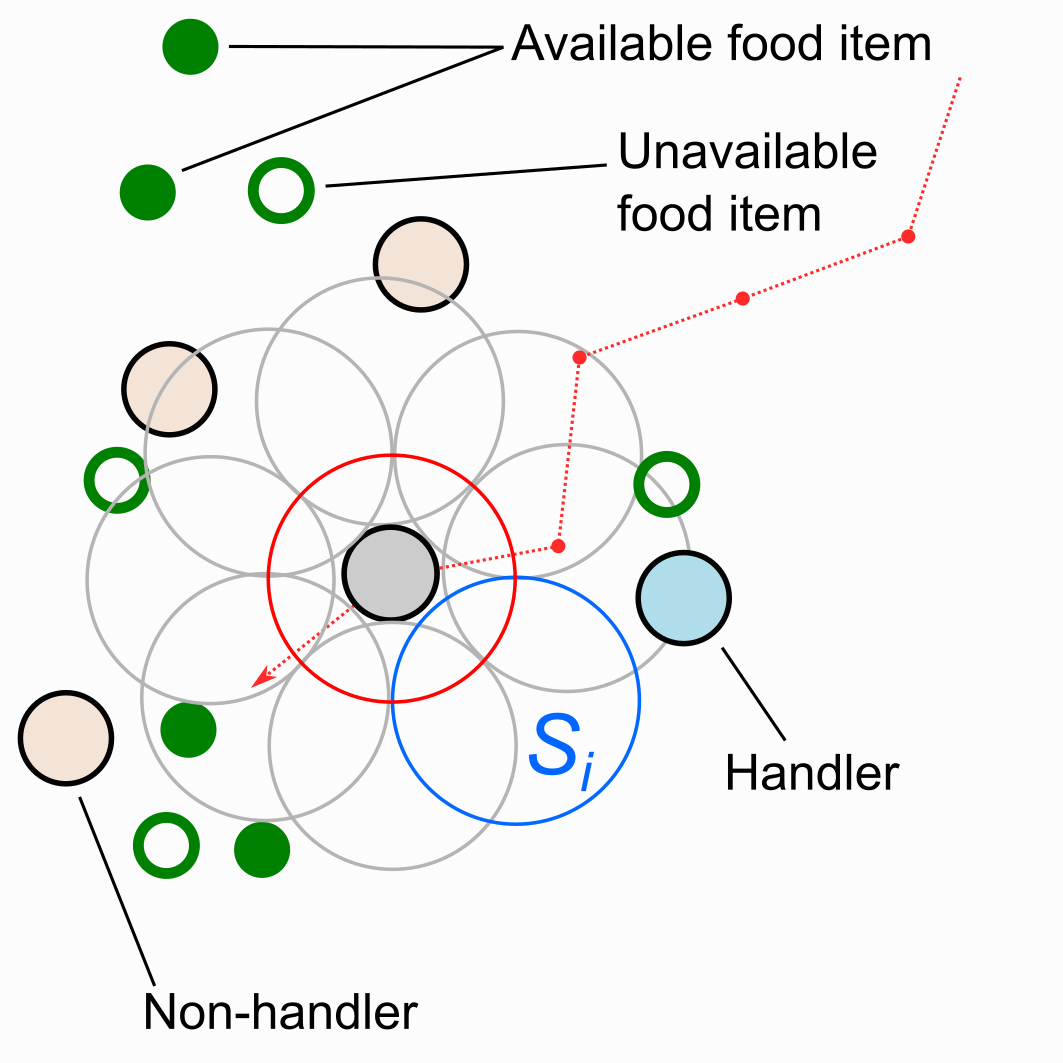
\includegraphics[width=0.9\linewidth]{figures/introduction/fig_schematic.png}
    \caption{
        \textbf{Schematic for a conceptual model of individual foraging movement as a series of discrete steps in continuous space, with movement steps selected based on individual preferences for environmental cues.} 
        In this model, individuals search for patchily distributed food items (\textbf{green circles}), which may be immediately available (\textbf{filled green circles}; \emph{F}), or may be available only in the future (\textbf{open green circles}). 
        Individuals can sense only available items, and not unavailable ones. However, as food items are clustered, available items are a good indirect indicator of where resource clusters are, and where items may become available in the future. 
        Individuals can also sense other foraging individuals, and can sense whether they have successfully found, and are handling, a food item (handlers; \textbf{blue circles}), or whether they are unsuccessful foragers still searching for food (non-handlers; \textbf{filled pink circles}; \emph{N}). 
        To decide where to move, individuals sample their environment for these three cues (\emph{F, H, N}) at their current location (\textbf{red circle}), and at a number of locations around themselves (\textbf{large open grey circles}; here, 8 locations). 
        When the sensory range is relatively large there is some small overlap in samples. 
        Individuals take their next step by assigning each potential direction a \emph{suitability}, \(S = s_FF + s_HH + s_NN + \epsilon\), where the coefficients \(s_F, s_H, s_N\) are individual preferences for environmental cues, and \(\epsilon\) is a small error term that helps break ties between locations.
        The individual cue preferences are numeric values, and can be treated as heritable properties to examine their evolutionary dynamics at the population level.
    }
    \label{fig:compare}
  \end{figure}

\subsection*{Random Walks and Optimal Movement}

In \textit{scenario 1}, individuals perform a random walk, and have a uniform probability of either remaining in their current location, or moving in a direction chosen from among eight locations within 1 distance unit (see Fig.~\ref{fig:compare}A); here, movement is independent of local cues.
In \textit{scenario 2}, individuals move in a way that is considered locally optimal in foraging ecology \citep{stephens2019,scherer2020}.
Each individual assesses local cues at its current location, and eight surrounding locations --- the number of available food items ($F$), and the number of potential competitors ($N + H$) --- and moves to the location with the highest potential intake pay-off, which is given by $(F / (N + H + 1)) + \epsilon$; $\epsilon$ is a small error term.
We initially contrast these two scenarios to show how adding semi-mechanistic decision making to individual movement can affect the outcomes of movement individual-based models.
As expected, optimally moving scenario 2 individuals had a higher per-capita intake than randomly moving scenario 1 individuals (Fig.~\ref{fig:compare}).
Individuals with higher intake should be expected to move less, as my model --- in line with foraging ecology theory \citep{charnov1976} --- explicitly considers a trade-off between movement and intake.
Surprisingly then, optimally moving individuals moved \textit{more} than random walkers (Fig.~\ref{fig:compare}).

Individuals in both scenarios had very similar numbers of spatial associations with other individuals (Fig.~\ref{fig:compare}, Fig.~\ref{fig:networks}).
Furthermore, these differences between movement scenarios were maintained on homogeneous landscapes as well (see SI Appendix X), contrary to the expectation that a more uniform spatial distribution of resources would allow random walkers to improve their outcomes, relative to optimal movement.
Overall, this comparison demonstrates the importance of active decision making in animal movement, and suggests why animals have evolved sophisticated sensory apparatuses to gather information from their environment \citep{avgar2013,berger2022,mann2021,swain2021}.
Such evolution is likely to be strongly dependent on fine-scale ecological conditions, primarily the \textit{availability} of information in the environment, as well as the energetic cost of evolving and maintaining sensory capabilities \citep{swain2021}.
However, one overlooked aspect in such models is how exactly individuals should incorporate local cues into movement decisions, which we tackle in the next two scenarios.

\subsection*{Movement as Mechanistic Decision-making}

Optimal movement models are often labelled mechanistic as they include environmental cues in decision making \citep[e.g.][]{scherer2020}, yet the potential payoff of a location is strongly influenced by the functional response of intake in relation to competitors --- this is often simply assumed by modellers \citep[][]{vandermeer1997}.
Such implementations make the implicit evolutionary assumption that all individuals weigh cues from their social and resource environments similarly, as such weighting is supposed to be the stable outcome of selection fine-tuning individuals' preferences.
However, the functional responses commonly used in foraging theory are often modelled on empirical data, and as such may not be properly generalisable to other eco-evolutionary contexts, nor sufficient to capture the mechanistic links between individuals' social environment, their behavioural decisions, and the consequences for intake.
I showcase a more mechanistic way in which individuals can determine their optimal step when making foraging movements, which is to have distinct preferences for local cues (food items and potential competitors).
These preferences are similar to the coefficients of habitat- and step-selection functions, which I introduce in the boxes below \citep[][]{fortin2005,avgar2013,thurfjell2014,avgar2016,fieberg2010,manly2007}.

\medskip

\begin{tcolorbox}[width=\textwidth,
    boxsep=0pt,
    left=0pt,
    right=0pt,
    top=2pt,
    arc=0pt,
    boxrule=0.0pt,
    toprule=1pt,
    bottomrule=1pt,
    colback=white
    ]%%
    \begin{description}
        \item[Step-selection Analysis: An Introduction] Step-selection analysis is a method developed from the study of empirical animal movement data, which seeks to determine the drivers of animal movement, with an early implementation in \textcite{fortin2005}'s study of the movement of deer in response to wolves, in Yellowstone National Park.
        In brief, step-selection analysis contrasts locations at which animals were observed, against locations that they could have used instead \parencite[][]{fortin2005}.
        The locations that are considered to have been available to an animal are conditioned upon its current location --- essentially, this avoids comparing used locations with distant regions that the animal could not have used at that time.
        In this sense step-selection analysis is essentially similar to conditional resource-selection analysis \parencite[see as general reference][]{manly2007}.
        The difference is that in step-selection analysis, the available locations are sampled from a distribution (usually the Gamma distribution) fitted to the movement distances obtained from the tracking data, with relative headings (`turning angles'; see \cite{calenge2009}) drawn from a von Mises distribution fitted to the animal's turning angles, again as seen in the tracking data \parencite[][]{thurfjell2014,signer2019}.
        The parameters determining the relative probability that a location is selected given its environmental attributes (the relative selection strengths, often denoted $\beta$) can be estimated via a maximum likelihood approach using common statistical software \parencite[see e.g. for R][]{therneau2000}.
        Overall, the probability that an animal will select a location is given by
        $$
            \hat{w}(x) = \text{exp}(\beta_1x_1 + \beta_2x_2 + \ldots \beta_nx_n)
        $$
        where $\hat{w}(x)$ is the selection score for a step, $\beta_i$ is the relative selection strength for (or against, if a negative value) the location attribute $x_i$.
    \end{description}
\end{tcolorbox}

\begin{tcolorbox}[width=\textwidth,
    boxsep=0pt,
    left=0pt,
    right=0pt,
    top=2pt,
    arc=0pt,
    boxrule=0.0pt,toprule=1pt,
    bottomrule=1pt,
    colback=white
    ]%%
    \begin{description}
        \item[Using Step-selection in Conceptual Models] Step-selection analysis is now widely used in animal movement ecology, with specialised implementations for habitat-specific movement characteristics \parencite{avgar2016}, decision points identified from very high-resolution data \parencite{munden2021}; it can also be extended to estimate animals' utilisation distributions \parencite{signer2017}.
        Indeed, recall that step-selection analysis is used even in this thesis (Chapter~\ref{ch:holeybirds}).
        Despite its popularity and ease of implementation, step-selection has seldom been used in individual-based simulation models of animal movement.
        One good example is \textcite{white2018}, who implemented a movement-disease model wherein individuals move across a grid, with their steps determined by their relative selection strengths ($\beta_i$) for cell attributes ($x_i$) such as resource levels or conspecific densities (in this sense they describe it as resource selection).
        In such models, individuals assign a selection score ($\hat{w}(x)$) to their current locations, and to neighbouring locations, and make the step with the highest score --- this may mean staying in place!
        Furthermore, $\beta_i$ values can be programmed to vary randomly or systematically in the population, to examine the effect of having individuals with a broad range of responses to similar cues (as \cite{white2018} do).
        In conceptual individual-based models such as mine, it is sufficient to denote the selection score (which I call `suitability') as
        $$
            S = \Sigma~s_{i}x_{i}
        $$
        where $S$, the selection score or suitability of the potential location, is simply the sum of the interaction of the individual's selection strengths (which I call a `preference'; $s_i$) and the value of the corresponding cue at that location ($x_i$).
        Given that the `cue preferences' are individual properties, they can be considered to be heritable between generations of a population, allowing the examination of evolutionary dynamics.
        This concept is examined further in the final scenario of my model, and models implementing this approach are described in Chapters~\ref{ch:kleptomove} and \ref{ch:pathomove}.
    \end{description}
\end{tcolorbox}

\subsection*{Examining Model Outcomes for Evolved Step-selection}

In my model's \textit{scenario 3}, individuals assesses local cues --- the number of available food items ($F$), and the number of potential competitors ($N + H$) --- at eight locations around themselves, and move to the location with the highest assessed suitability: $S = s_FF + s_C(N + H) + \epsilon$.
This is 
Here, $s_F$ and $s_C$ are inherited \textit{movement preferences} for food items and potential competitors respectively, and can take any positive or negative numeric values; $\epsilon$ is a small error term.
It is the relative contribution of $s_F$ and $s_C$ that determines individuals' \textit{movement strategy}.
I initialised the populations to have a broad range of movement strategies, so that it contained individuals with different combinations of preferences and avoidances of either food items or competitors.
Scenario 3 individuals had a lower median intake, and moved more overall, than individuals in scenarios 1 or 2.
As expected, intake was strongly positively correlated with the relative strength of individuals' preference for food items, $s_F$ (LMM coefficient here), while being uncorrelated with individuals' relative selection for competitors (LMM coefficient here).
Unsurprisingly then, scenario 3 populations were strongly clustered in space; however, they did not encounter substantially more individuals than scenario 2 individuals on average, although the variance in the number of encounters was large.

Given substantial inter-individual differences in intake based on relative preference for food items, biologists would expect that movement strategies that prefer food items would have a selection advantage.
I tested this expectation by adding an evolutionary component to the model: over 100 generations, individuals reproduce, passing on their preferences ($s_F$, $s_C$) to their offspring.
The preference values undergo random, independent mutations with a probability $p$ = 0.01, and with a mutation step size drawn from a Cauchy distribution with a scale of 0.01.
Consequently, most mutations are small, but larger mutations do occasionally occur.
The number of offspring is proportional to individuals' intake of food items during their lifetime \citep{netz2021,gupte2021a,gupte2022c}.
For simplicity, we assume asexual, haploid individuals, and that population sizes are fixed, and that generations do not overlap.
I implemented large-scale natal dispersal, such that individuals are typically initialised (`born') within a standard deviation of 10 units of their parents --- this makes scenario 3 relatively similar to the random initialisation of individual positions in scenarios 1 and 2 (but see SI Appendix 1 for an explanation of the outcomes under small-scale natal dispersal; see also \cite{gupte2021a,gupte2022c}).
These modelling choices must be explicitly implemented in simulation models' code, bringing the assumptions of classical models --- treated as received wisdom and hence ignored --- to the fore.

I found that scenario 3 population converged to a similar movement strategy within only a few (100) generations, across all twenty replicates.
This strategy was to primarily prefer moving towards food items, while having a small preference or avoidance of potential competitors.
The `evolved' scenario 3 individuals had better ecological performance than their ancestral populations (which we consider the first generation, G = 1), taking in more food items on average, and moving less.
Indeed, these populations outperformed both the random walk and optimal movement implementations as well.
Adapting their movement strategies to the landscape also affected the social structure of scenario 3 populations --- there were fewer isolated individuals, more spatial clustering, and consequently, individuals encountered more unique conspecifics on average (higher mean degree; Fig.~\ref{fig:networks}).

\subsection*{Adding Detail to Mechanistic Movement Decision-making}

A key feature of individual-based simulation models is their ability to incorporate great amounts of ecological detail \citep{deangelis2019}.
With a simple extension to scenario 3, we show how to add biologically relevant details to models, and how these details can affect model outcomes.
Foraging can be a form of public information, serving as an indirect cue of the presence of resources, and furthermore, helping distinguish between individuals that are \textit{immediate} competitors (here, non-handlers), and those which are only future potential competitors \citep[][; here, handlers]{dall2005,giraldeau2018,beauchamp2008,beauchamp2013}.
Thus in my \textit{scenario 4}, we allow individuals to sense the handling status of nearby potential competitors, and to have separate heritable preferences for handlers ($sH$) and non-handlers ($sN$).
Individuals assess the suitability of locations as $S = S = s_FF + s_HH + s_NN + \epsilon$; $\epsilon$ is a small error term.
I implemented similar evolutionary and dispersal dynamics as in scenario 3.

Individuals in the final generation (G = 200) of scenario 4 had mostly evolved a movement strategy that we describe as `handler tracking', i.e., having a preference for successful neighbours handling a food item ($sH >$ 0), but avoiding unsuccessful neighbours that were still searching for a food item \citep[($sN <$ 0)][]{gupte2021a,gupte2022c}.
This is similar to the scenario 2 `optimal movement' strategy, and allows individuals to avoid areas with many potential competitors, and thus a lower potential intake.
Importantly however, it allows individuals to use indirect social information \citep{dall2005,spiegel2016a}, in the form of the positions of successful neighbours, to find resource clusters --- even when these clusters are not immediately perceptible (due to earlier depletion).
Consequently, scenario 4 individuals outperform both scenario 1 and scenario 2 individuals by having substantially higher mean per-capita intake (Fig.~\ref{fig:compare}.
While not shown here, this naturally leads to the conclusion that the resource landscape in scenario 4 is more depleted than in scenarios 1 and 2.
Scenario 4 individuals, after 200 generations of selection, also outperform scenario 4 populations that have not undergone selection (i.e., their ancestors), demonstrating the difference that adding evolutionary dynamics makes even to a mechanistic, habitat selection model \citep[such as][]{white2018}.

Scenario 4 individuals' evolved use of social information on the potential locations of resource clusters also leads them to have more spatial associations with conspecifics --- indeed, up to three times as many as in the random walk and optimal movement models (Fig.~\ref{fig:compare}).
These associations likely occur at or near resource clusters, leading to substantial spatial-social clustering in the final generation of scenario 3 populations (Fig.~\ref{fig:networks}).
Scenario 4 individuals across replicates associated with more individuals (degree, mean $\pm$ SD = ) than in scenarios 1, 2 and 3.
Spatial-social structure in animal populations can have important consequences for a wide range of processes and phenomena in animal ecology, including the transmission of animal culture \citep[such as foraging tactics or migration routes][]{romano2020,romano2021,jesmer2018,klump2021}, as well as the spread of infectious pathogens \citep{white2017,white2018,white2018b,webber2022,ezenwa2016,albery2020}.

\begin{figure}[!h]
    \centering
    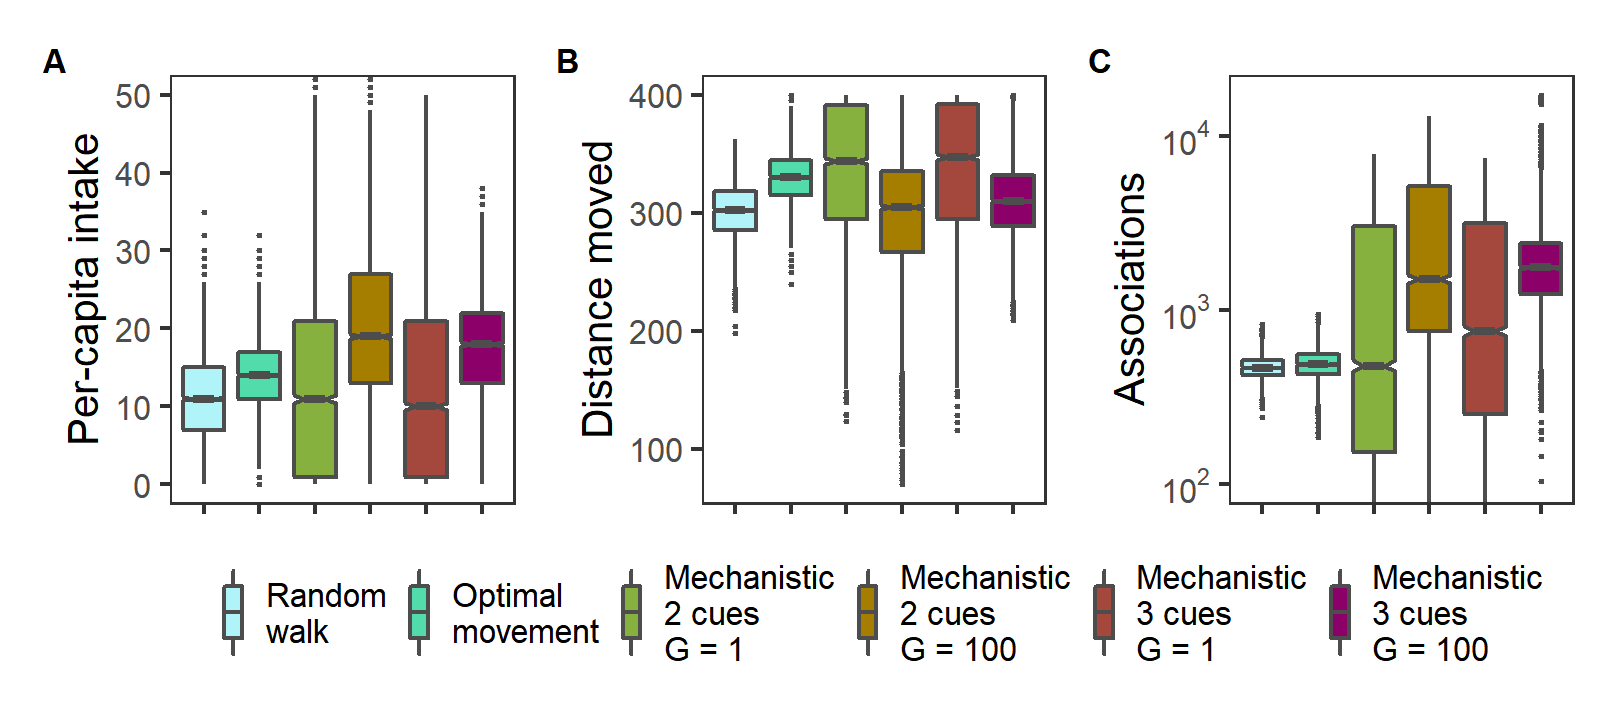
\includegraphics[width=0.95\linewidth]{figures/introduction/fig_cs_2_1.png}
    \caption{
        \textbf{Differences in population ecological outcomes emerge from differences in the implementation of movement in individual-based simualtion models.}
        \textbf{(A)} In \textit{scenario 1}, individuals moving randomly across the landscape had expectedly lower per-capita intake than individuals moving in a locally optimal way (\textit{scenario 2}).
        Surprisingly, optimal movers also moved more than random walkers, with no apparent trade-off between movement and intake \textbf{(B)}.
        When individuals selected their movement step based on heritable movement preferences for food items and conspecific competitors (\textit{scenario 3, `mechanistic 2 cues'}; A), they had a wide variance in intake, with the population median equivalent to that achieved by a random walk.
        However, after only 100 generations of natural selection for adaptive movement preferences, scenario 3 populations had a higher intake than ostensibly `optimal' movement.
        Allowing individuals to differentiate between current and future competitors (non-handlers and handlers, respectively; \textit{scenario 4, `mechanistic 3 cues'}), did not improve individuals' intake, suggesting that relatively simple mechanistic movement strategies may suffice on even complex, fluctuating resource landscapes.
        \textbf{(C)} Movement implementations strongly influenced individuals' associations (based on proximity), with mechanistic movement leading to many times more associations than random or optimal movement.
    }
    \label{fig:compare}
    \end{figure}

\begin{figure}[p]
    \centering
    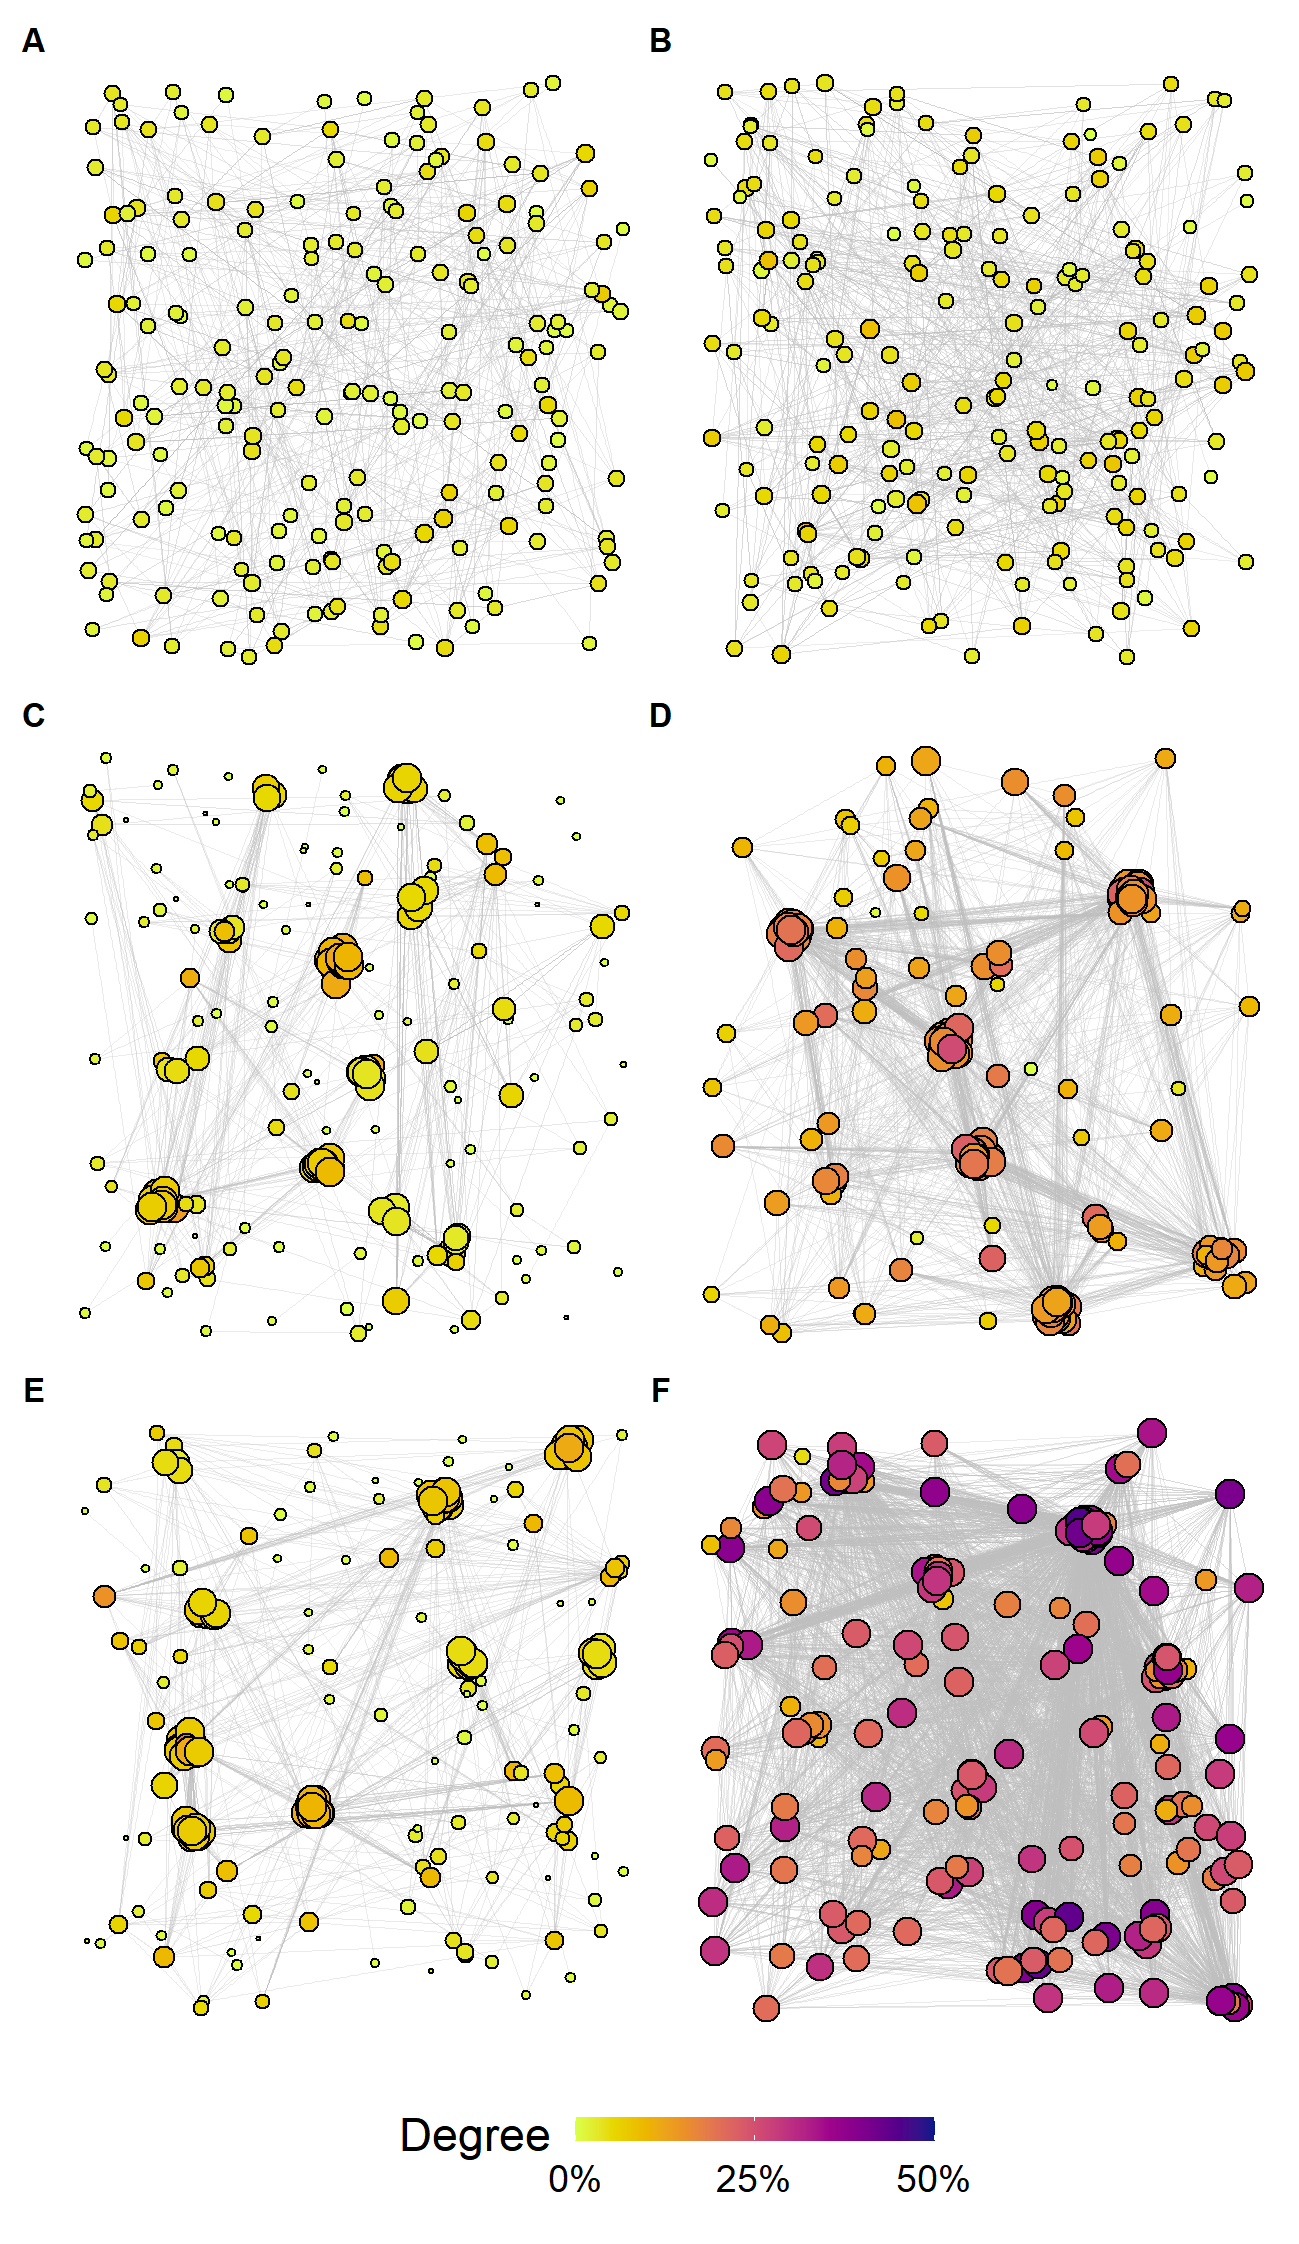
\includegraphics[width=0.9\linewidth]{figures/introduction/fig_cs_2_networks.png}
    \caption{
        \textbf{Differences in movement implementations lead to substantially different patterns of spatial-social associations.}
        Individuals moving randomly (\textbf{A}: scenario 1), or in semi-mechanistic, optimal ways (\textbf{B}: scenario 2) have sparse social networks, with individuals spread out over the simulated resource landscape.
        Most individuals have a low degree, i.e., few unique social partners.
        In contrast, individuals making mechanistic movement decisions based on two cues (food and competitors; \textbf{C}: scenario 3) have much more spatially clustered networks, with a substantially higher mean degree (more unique social partners).
        Over 100 generations, scenario 3 individuals are selected for their preference for food items, and the resulting populations form networks that are also clustered, but with strong connectivity between clusters, and more unique partners overall \textbf{(D)}.
        A similar dynamic is seen in scenario 4, where initially, populations have a wide diversity of movement strategies, leading some individuals to avoid associations \textbf{(E)}. After 100 generations, most individuals still avoid immediate competitors (non-handlers), leading to more dispersed populations than scenario 3, though with strong links between nodes.
    }
    \label{fig:networks}
  \end{figure}

\subsection*{Emergent Model Properties: Consequences for Disease Transmission}

To examine the consequences for disease ecology, I began by constructing social networks by recording individuals' pairwise associations (distance $<$ perception range) in all four scenarios \citep{farine2015}.
I ran simple epidemiological models with SIR assumptions over the social networks emerging in each scenario \citep[25 replicates per network; 1 network per scenario replicate][]{white2017,csardi2006,bailey1975}, with a hypothetical disease (transmission probability $\beta$ = 2.0, recovery probability $\gamma$ = 1.0; see Fig.~\ref{fig:sir}).
Between the non-mechanistic scenarios, the disease spread more rapidly through networks arising from the optimal movement model, than the random walk model.
In scenario 3, the disease spread much more rapidly through the population after selection for movement preferences (G = 100), than through the ancestral population that had not undergone such selection (G = 1), despite both populations being similarly spatially clustered.
This is not unexpected as initially (G = 1), there are a number of individuals that avoid potential competitors ($s_C <$ 0), and this could hinder transmission in comparison with their descendants, fewer of which are similarly isolated.
Importantly, the unevolved mechanistic movement implementation had a lower infection peak than the random walk and optimal movement implementations.
A model beginning with diverse movement strategies, and not including an evolutionary component when implementing mechanistic movement \citep[such as][]{white2018}, would correctly conclude that mechanistic movement implementations differ from more mainstream movement modelling approaches in epidemiological outcomes, but crucially miss that this difference is that a disease would spread much more rapidly through the population.
Scenario 4 obtains a similar result --- populations adapted to their landscape cluster together, which allows a disease to spread even faster through their network than in scenario 3.

\begin{figure}[!h]
    \centering
    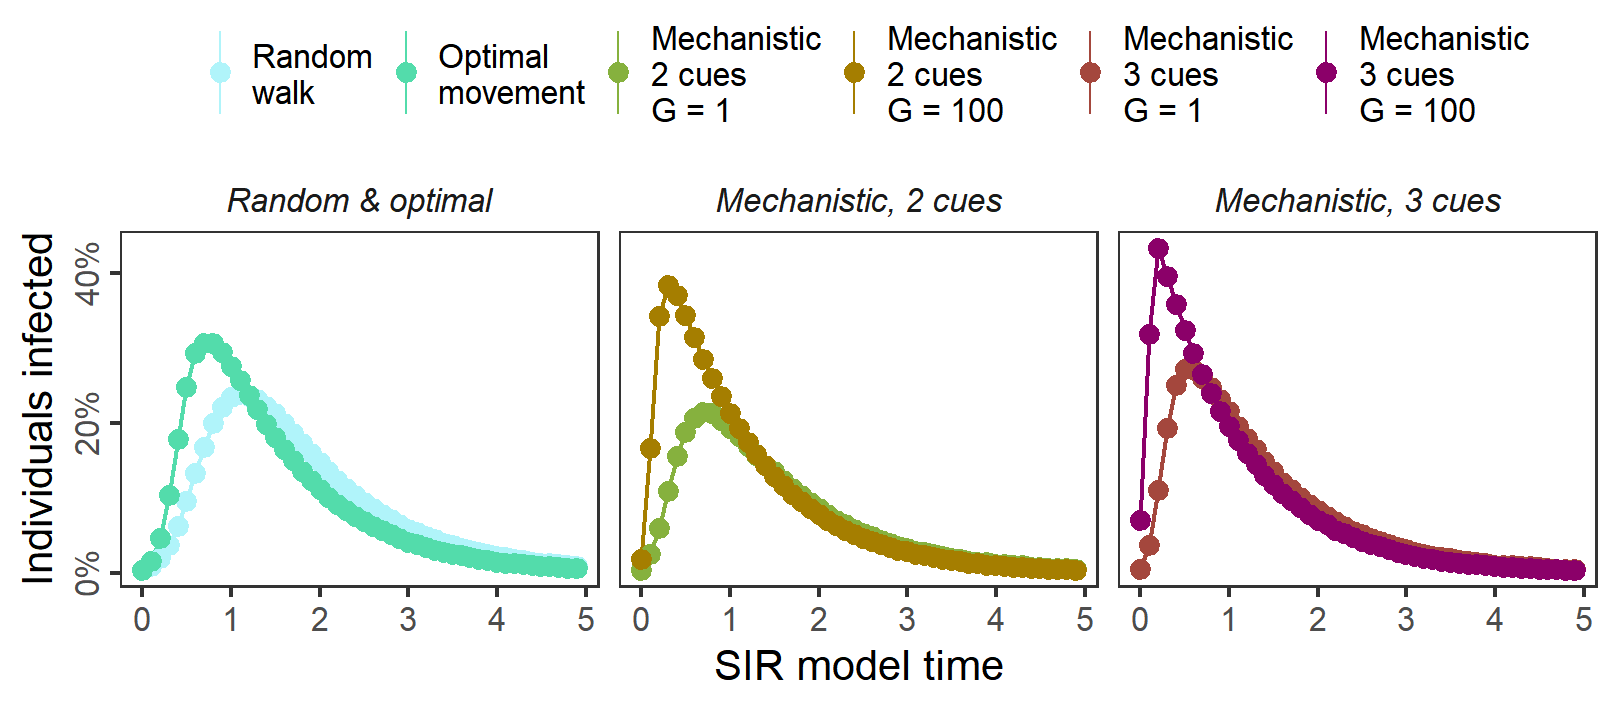
\includegraphics[width=0.9\linewidth]{figures/introduction/fig_cs_2_2.png}
    \caption{
        \textbf{Case study 2: Effect of movement implementations on the outbreak of hypothetical disease.}
        Modelling a disease outbreak using a simple SIR model conditioned on the social networks of each population (e.g. as shown in Fig.~\ref{fig:networks}) shows that how movement is implemented in models can strongly influence epidemiological conclusions (disease transmission rate $\beta$ = 2.0, recovery rate $\gamma$ = 1.0).
        \textbf{(A)} The hypothetical disease spreads more rapdily through \textit{scenario 2} than \textit{scenario 1}, as scenario 2 networks are somewhat better connected. This is likely because optimal movement is better at leading individuals towards resource clusters where they must associate with conspecifics while feeding.
        \textbf{(B)} Modelling movement as mechanistic step-selection based on preferences for local cues (\textit{scenario 3}: mechanistic, 2 cues) leads to drastically different conclusions depending on whether the model includes an evolutionary component. Diseases spread less rapidly through ancestral populations with a diversity of movement strategies, than through populations moving optimally or even randomly.
        However, after 100 generations of selection, the population has primarily social agents that are strongly inter-connected, leading to very rapid disease outbreaks.
        \textbf{(C)} Disease dynamics are similar in \textit{scenario 4} (mechanistic, 3 cues): the spread of disease through initial networks (G = 1), is not representative of the spread through populations that have undergone selection (G = 100).
    }
    \label{fig:sir}
  \end{figure}

Overall, individual-based models offer the potential for more realistic social networks to emerge, with the expectation of more robust epidemiological insights from these networks \citep[][]{lunn2021}.
The development of spatially explicit movement-disease models allows both movement and disease transmission dynamics to be modelled explicitly \citep{white2018b,white2018,scherer2020,gupte2022c}.
However, network models conditioned on emergent social networks allow multiple pathogen scenarios to be run on the same network, saving computational time, and they also enable comparison with empirical work in the disease ecology of moving animals \citep{wilber2022}.
The importance of network formation processes in epidemiological modelling is already well known \citep[][]{white2017,wilber2022}.
My example model demonstrates how social networks emerging from individual-based movement models are sensitive to the modelling of the movement process, and how model details can affect predictions about disease outbreaks, and animal spatial-social ecology generally \citep{webber2018,webber2022}.
Furthermore, including evolutionary dynamics in combined movement-disease models can reveal surprisingly rapid evolutionary transitions in social movement strategies that make populations more robust to the spread of pathogens (see Chapter~\ref{ch:pathomove}).

{ \begin{center} \barfont{-.-} \end{center} }

\endgroup

\clearpage
